\documentclass{article}

\usepackage{amsmath}
\usepackage{amsthm}
\usepackage{amssymb}
\usepackage{graphicx}

\graphicspath{{pics/}}

%CURLIES  :)       $\{$ $\}$

\newcommand{\ti}[1]{\textit{#1}}
\newcommand{\N}{\mathbb{N}}
\newcommand{\Z}{\mathbb{Z}}
\newcommand{\Q}{\mathbb{Q}}
\newcommand{\R}{\mathbb{R}}
\newcommand{\C}{\mathbb{C}}
\newcommand{\bbP}{\mathbb{P}}
\newcommand{\Om}{\Omega}
\newcommand{\om}{\omega}
\newcommand{\emp}{\emptyset}
\newcommand{\lt}{\textless}
\newcommand{\gt}{\textgreater}
\newcommand{\imply}{\Rightarrow}

\title{MATH 323 Class Notes}
\author{Owen Lewis}
\date{Summer 2018}

\begin{document}
\begin{titlepage}
\maketitle
\end{titlepage}

\tableofcontents
\newpage

%%%%%%%%%%%%%%%%%%%%%%%%%%%%%%%%%%%%%%%%%%%%%%%%%%%%%%%%%%%%%%%%%%%%%%

\section{May 1, 2018}
\subsection{Definitions}
Let $\Omega$ be the set of all possible outcomes. We call $\Omega$ the $\ti{Sample Space}$.\\\\
\textbf{Ex 1:} Flipping a coin. The possible outcomes are $H$ and $T$\\
$\imply$ $\Omega$ = $\{$$H$, $T$$\}$.\\
\textbf{Ex 2:} Tossing a die. We list all the outcomes as $\omega_{i}$ where $i$ is the face of the die that we land on. We'll assume a normal 6-sided die\\ 
$\imply$ $\Omega$ = $\{$$\omega_{1}$, $\omega_{2}$,\dots, $\omega_{6}$$\}$.\\
\textbf{Ex 3:} Flipping a coin until an $H$ appears. The possible outcomes are $H$, $TH$, $TTH$,\dots, $TT$$\dots$$TH$ (with $n-1$ $T$s), $\dots$ ad infinitum.\\\\
$\imply$ $\Omega$ = $\{$$H, TH, TTH, TTTH, TTTTH,\dots$$\}$.\\
Note that in this case, $\Omega$ is a (countably) infinite set!\\\\
Let $\Omega$ be a sample space. Any subset $A$ of $\Omega$ is called an $\it{Event}$.
\begin{itemize}
	\item If $A$ = $\emptyset$, then we call $A$ the $\ti{Null Event}$
	\item If $A$ = $\Omega$, then we call $A$ the $\ti{Certain Event}$
	\item If $|$$A$$|$ = 1, then we call $A$ an $\ti{Elementary Event}$
\end{itemize}
\textbf{Ex:} Tossing a die. Let $\Omega$ := $\{$$\omega_{1}$, $\omega_{2}$,\dots, $\omega_{6}$$\}$, $A$ := $\{$$\omega_{1}$, $\omega_{2}$$\}$. Then $A$ is an event but is not an elementary event.\\\\
If $A$ is an event, then $A^{c}$ is also an event called the $\ti{complement event}$ of $A$.\\
If $A, B$ are two disjoint events then we call $A$, and $B$ $\ti{mutually exclusive}$, or $\ti{disjoint}$.\\\\
Let $\Omega$ be a sample space, $\mathcal{P}$ be the power set of $\Om$. A $\ti{Probability}$ $\bbP$ on $\Om$ is a function $\bbP$ : $\mathcal{P}$($\Om$) $\rightarrow$ [0, 1], such that:
\begin{enumerate}
	\item $\forall$ $A$ $\subseteq$ $\Om$, 0 $\leq$ $\bbP$($A$) $\leq$ 1
	\item $\bbP$($\Om$) = 1
	\item If $A_{1}$, $A_{2}$,\dots, $A_{n}$,\dots\ is a sequence of pairwise disjoint events then
\[ \bbP(\bigcup_{i=1}^{\infty} p_{i}) = \sum_{i=0}^{\infty} \bbP(A_{i}) \]
\end{enumerate}
\newpage
\subsection{How do we Apply this?}
Let $\Om$ be a discrete set, $E_{i}$ = $\{$$\omega_{i}$$\}$ be an elemental event, with $E_{i}$ $\subseteq$ $\Om$. A probability on $\Om$ is given by a sequence $\bbP_{1}$, $\bbP_{2}$,\dots, $\bbP_{n}$,\dots of positive numbers such that
\[ \bbP(E_{i}) = p_{i},\ and\ \sum_{i} \bbP(p_{i}) = 1\]\\
If $A$ $\subseteq$ $\Om$, then
\[ \bbP(A) = \sum_{\omega_{i} \in A} \bbP(p_{i})\]\\
\textbf{Ex 1:} Toss a die.\\
a) Given that $\bbP$($\omega_{2}$) = $\bbP$($\omega_{4}$) = $\bbP$($\omega_{5}$) = $\bbP$($\omega_{6}$) = $\frac{1}{6}$, $\bbP$($\omega_{1}$) = $\frac{1}{4}$, find $\bbP$($\omega_{3}$).\\
b) Find the probability that the die will land on an odd face.\\
\textbf{Solution:}\\
a) $\Omega$ = $\{$$\omega_{1}$, $\omega_{2}$,\dots, $\omega_{6}$$\}$. $\bbP$($\omega_{3}$) is a singleton, and as we know $\sum_{i} \bbP(p_{i})$ = 1 then  $\sum_{i=1}^{6}\bbP(\omega_{i})$ = 1 $\implies$ $\bbP$($\omega_{2}$) + $\bbP$($\omega_{4}$) + $\bbP$($\omega_{5}$) + $\bbP$($\omega_{6}$) + $\bbP$($\omega_{1}$) + $\bbP$($\omega_{3}$) = 1 $\implies$ $\frac{4}{6}$ + $\frac{1}{4}$ + $\bbP$($\omega_{3}$) = 1 $\implies$ $\bbP$($\omega_{3}$) = 1 - $\frac{11}{12}$\\
$\implies$ $\bbP$($\omega_{3}$) = $\frac{1}{12}$.\\
b) Let $A$ $\subseteq$ $\Om$ be the subset of $\Om$ containing all the odd faces. The total probablilty of $A$ is therefore the sum of all the probabilities of the elements of $A$ $\imply$ $\bbP$($A_{i}$) = $\frac{1}{4}$ + $\frac{1}{12}$ + $\frac{1}{6}$ = $\frac{1}{2}$.\\\\
\textbf{Ex 2:} Given a countably infinite sample space, find a constant $c$ such that $\bbP$($\{$$\omega_{n}$$\}$) = $c(\frac{1}{5})^n$ for some $n$.\\
\textbf{Solution:} $\sum_{n=1}^{\infty} \bbP$($\{$$\omega_{n}$$\}$) = 1 $\imply$ $\sum_{n=1}^{\infty} c(\frac{1}{5})^n$ = 1 $\imply$ $\sum_{n=1}^{\infty} (\frac{1}{5})^n$ = $\frac{1}{c}$. Notice how $\sum_{n=1}^{\infty} (\frac{1}{5})^n$ is a geometric series that converges to $\frac{1}{4}$ $\imply$ therefore $\frac{1}{c}$ = $\frac{1}{4}$\\
$\imply$ $c$ = 4.
\newpage

%%%%%%%%%%%%%%%%%%%%%%%%%%%%%%%%%%%%%%%%%%%%%%%%%%%%%%%%%%%%%%%%%%%%%%

\section{May 2, 2018}
\subsection{Properties of $\bbP$}
Let $\Om$ be a sample space and let $\bbP$ be a probability on $\Om$. Then:
\begin{enumerate}
	\item $\bbP$($\emptyset$) = 0
	\item $\bbP$($A^{c}$) = 1 - $\bbP$($A$)
	\item $\bbP$($A \cup B$) = $\bbP(A)$ + $\bbP(B)$ - $\bbP(A \cap B)$
\end{enumerate}
Proof:
\begin{enumerate}
	\item Set $A_{1}$ = $\Om$, $A_{2}$ = $\emp$. Then $A_{1} \cup A_{2}$ = $\Om$, and $A_{1} \cap A_{2}$ = $\emp$. Therefore $\bbP(A_{1} \cup A_{2}$) = $\bbP(A_{1})$ + $\bbP(A_{2})$ $\imply$ $\bbP(\Om)$ = $\bbP(\emp)$ + $\bbP(\Om)$ $\imply$ 1 = $\bbP(\emp)$ + 1\\ $\imply$ 0 = $\bbP(\emp)$. \qed

	\item $A^{c} \cup A$ = $\Om$, and $A^{c} \cap A$ = $\emp$. Then = $\bbP(\Om)$ $\imply$ 1 = $\bbP(A^{c} \cup A)$\\ $\imply$ 1 = $\bbP(A)$ + $\bbP(A^{c})$ $\imply$ $\bbP(A^{c})$ = 1 - $\bbP(A)$. \qed

	\item It's easy to show that $A$ = $(A \setminus B) \cup (A \cap B)$, and $\emp$ = $(A \setminus B) \cap (A \cap B)$. Similarily, $\bbP(A)$ = $\bbP(A \setminus B)$ + $\bbP(A \cap B)$. From these, it follows that\\ $A \cup B$ = $A \cup (B \setminus A)$ $\imply$ $\bbP(A \cup B)$ = $\bbP(A)$ + $\bbP(B \setminus A)$\\ $\imply$ $\bbP$($A \cup B$) = $\bbP(A)$ + $\bbP(B)$ - $\bbP(A \cap B)$. \qed
\end{enumerate}

\subsection{Equiprobability}
Let $\Om$ be a finite sample space. Set $N$ := $|\Om|$. Equiprobability means that all outcomes have the same probability $\bbP$ = $\frac{1}{N}$. Let $A \subseteq \Om$ be an event. Then we have $\bbP(A)$ = $|A|$$\cdot$$\frac{1}{N}$, or 
\[\bbP(A) = \frac{|A|}{|\Om|}\]
This is great because it means that in \textbf{equiprobability} problems we just need to count the cardinality of $A$, count the cardinality of $\Om$, and divide them, and we're done. Too bad counting isn't really all that easy.

\subsection{Counting Tools}
We have here three tools to help us calculate the cardinalities of huge (finite) subsets of huge sample spaces, each with their own specific situations that require its use
\begin{enumerate}
	\item The Cartesian Product
	\item Permutations
	\item Combinations
\end{enumerate}
\subsubsection{The Cartesian Product}
\paragraph{}
We all know what the cartesian product $is$. In probability we use it in our experiment when we have more than one """input""" each with its own possible outcome, for example, we roll three dice, or flip two coins.
\paragraph{}
Let $A$, $B$, be sets such that $|A|$ = $a$, and $|B|$ = $b$. Then the cardinality of the cartesian product $|(A \times B)|$ is $|(A \times B)|$ = $a \cdot b$.\\\\
\textbf{Ex 1:} Suppose we roll a die twice. What is the cardinality of the sample space $\Om$?\\
\textbf{Solution:} If we roll a die once we have $\Om$ = $\{$$\omega_{1}$, \dots, $\omega_{6}$$\}$. Therefore, the sample space for rolling a die twice is $\Om \times \Om$. The cardinality of our sample space $\Om \times \Om$ is $|\Om \times \Om|$ = 6 $\cdot$ 6 = 36.\\\\
\textbf{Ex 2:} Suppose we roll a fair die twice. What is the probability that the outcome is even?\\
\textbf{Solution:} If the sum of the two outcomes is even then both must either be even or both must be odd. Let $A$ be the event where the sum of the rolls is even, and let $A_{1}$ be event where both individual rolls are even, $A_{2}$ be the event where both individual rolls are odd. For example,
\[A_{1} = \{(2, 2), (2, 4), (2, 6), (4, 2), (4, 4), (4, 6), (6, 2), (6, 4), (6, 6)\}\] 
Where the 1$^{st}$ element in each ordered pair is the outcome of the 1$^{st}$ roll and the 2$^{nd}$ element in each ordered pair is the outcome of the 2$^{nd}$ roll. Therefore, we have that $|A_{1}|$ = $|A_{2}|$ = 9.\\ 
Since naturally $A$ = $A_{1} \cup A_{2}$ then $\bbP(A)$ = $\bbP(A_{1})$ + $\bbP(A_{2})$. We also know that the die was fair, so we can use our equiprobability formula here.
\[ \bbP(A) = \bbP(A_{1}) + \bbP(A_{2}) = \frac{|A_{1}|}{|\Om|} + \frac{|A_{2}|}{|\Om|} = \frac{9}{36} + \frac{9}{36} = \frac {18}{36} = \frac{1}{2}.\]
\subsubsection{Permutations}
A permutation of $r$ integer elements chosen from $n$ (possible elements) is equivalent to a successive draw, without replacement, of $r$ elements from a list of $n$ elements. We denote the number of possibilities by $P_{r}^{n}$. The general formula for $P_{r}^{n}$ is
\[P_{r}^{n} = n \cdot (n-1) \cdot \dots \cdot (n-r+1) = \frac{n!}{(n-r)!}\]\\
\textbf{Ex:} \\
a) A thick black bag contains 4 balls: 1 green, 1 blue, 1 red, 1 yellow. The bag is made of lead, or something, and also light cannot exist in this bag. You couldn't see into this bag if your life depended on it. Draw successively two balls from the bag without putting them back in. What is the probability that the second ball drawn is green?\\
b) What is the probability that one of the two balls drawn will be green?\\
\textbf{Solution:}\\
a) Let $\Om$ be the set of permutations of 2 balls chosen from the bag containing 4 balls. Then, $|P^{4}_{2}|$ = $\frac{4!}{2!}$ = $\frac{24}{2}$ = 12. Then let $A$ be the event where the second ball is green. The cardinality of $A$ is 3, as if we take for granted that the second ball is green, then there are 3 other different-coloured balls in the bag to accompany it. Since the bag is so dark that it's physically impossible to see inside it, all the balls in the bag have an equal probability of being drawn. Therefore,
\[ \bbP(A) = \frac{|A|}{|\Om|} = \frac{3}{12} = \frac{1}{4}\]
b) Let $B$ be the event where one of the balls drawn is green. Suppose $B_{1}$ is the event where the first ball drawn is green, and $B_{2}$ is the event where the second ball drawn is green. In part a) we found that $|B_{2}|$ = 3, and a parallel argument shows that $|B_{2}|$ = 3 as well. Thus,
 \[ \bbP(B) = \frac{|B_{1}|}{|\Om|} + \frac{|B_{2}|}{|\Om|} = \frac{3}{12} + \frac{3}{12} = \frac{6}{12} = \frac{1}{2}\]
\subsubsection{Combinations}
Consider a set $\Om$ with $n$ elements. Let $r$ be an integer such that $0 \leq r \leq n$. A combination $C^{n}_{r}$, also denoted ${n}\choose{r}$ (pronounced $n$ choose $r$), is the number of subsets of $\Om$ containing $r$ elements. The general formula is
\[C^{n}_{r} = \frac{P_{n}^{r}}{r!} = \frac{n!}{r! \cdot (n-r)!}\]
\textbf{Ex:}\\
a) Out of a deck of 52 cards how many distinct 5-card hands are possible?\\
b) What is the probability that a given hand contains at least one ace?\\
\textbf{Solution:}\\
a) ${52}\choose{5}$ = $\frac{52!}{5! \cdot (47!)}$ = 2,598,960\\
b) In this case it is easier to calculate the probability where the hand contains no aces and then subtract that from 1 to find the probability that we have an ace. If $A$ is the event where the hand contains an ace, then $A^{c}$ is the event where a hand contains no ace. Then
\[\bbP(A^{c}) =  \frac{|A^{c}|}{|\Om|} = \frac{C^{48}_{5}}{C^{52}_{5}} = \frac{1,712,304}{2,598,960} = \frac{35,673}{54,145}\]
Then we need to subtract this from 1 and we're done
\[\bbP(A) = 1 - \frac{35,673}{54,145} \approx 0.3412\]
\subsection{Properties of Combinations}
Here are some properties of combinations
\begin{enumerate}
	\item $C^{n}_{0}$ = $C^{n}_{n}$ = 1
	\item $C^{n}_{r}$ = $C^{n}_{n-r}$ $0 \leq r \leq n$
	\item $C^{n}_{r}$ = $C^{n-1}_{r}$ + $C^{n-1}_{r-1}$ $0 \leq r \leq n$
\end{enumerate}
The proofs are really easy and I dont wan't to bother typing them out but here is the idea behind each of them:
\begin{enumerate}
	\item Trivial
	\item Induction on $n$
	\item Also induction on $n$
\end{enumerate}
\subsubsection{Pascal's Triangle}
Pascal's triangle is a table of combinations $C_{r}^{n}$. The rows of the triangle represent $n$, starting at 0 at the tip and working down, and the $r^{th}$ element from the left (starting at 0) represents $r$. Each number in the triangle is determined by summing the two numbers directly above it.\\
\begin{center}
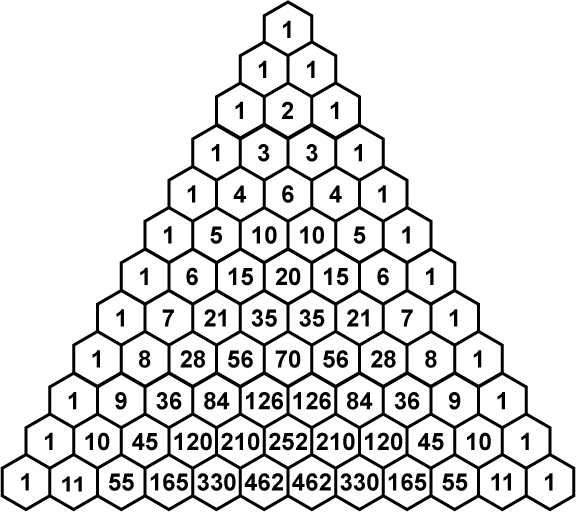
\includegraphics[scale=0.5]{pascal.png}\\
\textit{Pascal's Triangle}
\end{center}
\newpage

%%%%%%%%%%%%%%%%%%%%%%%%%%%%%%%%%%%%%%%%%%%%%%%%%%%%%%%%%%%%%%%%%%%%%%

\section{May 3, 2018}
\subsection{Binomial Theorem}
$(a+b)^{n}$ = $\sum_{k=0}^{n} C_{k}^{n} \cdot a^{k} \cdot b^{n-k}$\\\\
\textbf{Ex 1:} $(a+b)^{3}$ = $C_{0}^{3} \cdot a^{6}b^{3}$ + $C_{1}^{3} \cdot ab^{2}$ + $C_{2}^{3} \cdot a^{2}b$ + $C_{3}^{3} \cdot a^{3}b$ = $b^{3} + 3ab^{2} + 3ba^{3} + a^{3}$\\\\
\textbf{Ex 2:} Find the coefficient of $x^{6}$ in the expansion of $(x^{2}+2)^{7}$.\\
\textbf{Solution:} If we let $x^{2}$ := $a$ and 2 := $b$, then from the binomial theorem:
\[(a+b)^{n} = \sum_{k=0}^{n} C_{k}^{n} \cdot a^{k} \cdot b^{n-k} = \sum_{k=0}^{n} C_{k}^{7} \cdot a^{k} \cdot b^{7-k} = C_{3}^{7} \cdot 2^{4} = 560\]
\subsection{Conditional Probability}
Let $\Om$ be a sample space and let $\bbP$ be a probability on $\Om$. Let $A \subseteq \Om$ be an event such that $\bbP(A)\ \gt\ 0$, and let $B \subseteq \Om$ be another event. The \textit{conditional probability of $B$ given $A$}, is defined as
\[ \bbP(A|B) = \frac{\bbP(B \cap A)}{\bbP(A)}\]\\
$\textbf{Ex 1:}$ We have 2 urns. Urn 1 contains 7 red balls and 4 blue balls, and urn 2 contains 5 red balls and 6 blue balls. First, we choose a ball from urn 1 and place it into urn 2, then we remove a ball from urn 2. What is the probability that the ball that we remove from urn 2 will be blue?\\
\textbf{Solution:} Let $B$ be the event where the ball drawn from urn 2 is blue, and let $A_{r}$, $A_{b}$ be the events where we draw a red or a blue ball from urn 1 respectively. Then $\bbP(A_{r})$ = $\frac{7}{11}$ and $\bbP(A_{b})$ = $\frac{4}{11}$. Also,
\[B = B \cap \Om \iff B = B \cap (A_{r} \cup A_{b}) \iff B = (B \cap A_{r}) \cup (B \cap A_{b})\]
Which then implies
\[\bbP(B) = \bbP(B \cap A_{r}) + \bbP(B \cap A_{b}) \iff \bbP(B) = \bbP(B|A_{r}) \cdot \bbP(A_{r}) + \bbP(B|A_{b}) \cdot \bbP(A_{b})\]
So all that is left is to compute $\bbP(B|A_{r})$, and $\bbP(B|A_{b})$.\\
From the definition, we can see that $\bbP(B|A_{r})$ = $\frac{1}{2}$, and $\bbP(B|A_{b})$ = $\frac{7}{12}$, so finally
\[ \bbP(B) = \frac{6}{12} \cdot \frac{7}{11} + \frac{7}{12} \cdot \frac{4}{11} = \frac{70}{132} \]\\
\textbf{Ex: 2} Roll a fair die. Let $A \subseteq \Om$ be the event where the outcome is even, $B \subseteq \Om$ be the event where the outcome is odd, $C \subseteq \Om$ be the event where the outcome is either a 1 or a 2. Compute all the conditional probabilities.\\
\textbf{Solution} First $\bbP(A) = \frac{1}{2}$, $\bbP(B) = \frac{1}{2}$, and $\bbP(C) = \frac{1}{3}$ Then:\\
$\bbP(A|B) = \frac{\frac{1}{6}}{\frac{1}{2}}$ = $\frac{1}{3}$, and $\bbP(B|A) = \frac{\frac{1}{6}}{\frac{1}{2}}$ = $\frac{1}{3}$\\
$\bbP(A|C) = \frac{1}{2}$, and $\bbP(C|A) = \frac{1}{3}$\\
$\bbP(B|C)$ = 1, and $\bbP(C|B) = \frac{2}{3}$\\
\subsection{Independent Events}
Let $A$, and $B$ be two events over some sample space $\Om$. $A$, and $B$ are said to be $independent$ if and only if:
\begin{enumerate}
	\item $\bbP(A|B)$ = $\bbP(A)$
	\item $\bbP(B|A)$ = $\bbP(B)$
	\item $\bbP(A \cap B)$ = $\bbP(A)$ $\cdot$ $\bbP(B)$
\end{enumerate}
\textbf{Ex: }\\ 
a) From the previous example, are $A$ and $B$ independent? \\
b) What about $A$ and $C$?\\
c) $B$ and $C$?\\
\textbf{Answers:}\\
a) No.\\
b) Yes.\\
c) No.\\
\subsection{Baye's Rule}
Let $A, B \subseteq \Om$ be events on a sample space $\Om$. Then the equation
\[ \bbP(A|B) = \frac{\bbP(B|A) \cdot \bbP(A)}{\bbP(B)}\]
is calles Baye's Rule, or Baye's Theorem.\\\\
\textbf{Theorem:} Total Probability Rule\\ 
Let $\Om$ be a sample space, and let $A \subseteq \Om$ be an event. Suppose we partition $\Om$ like $\Om$ = $\{$$B_{1}, B_{2}, \dots, B_{n}$$\}$, where the $B_{i}$s are pairwise disjoint events such that
\[ \bigcup_{i=1}^{n}B_{i} = \Om\]
Then:
\begin{enumerate}
	\item $\bbP(A)$ = $\sum_{i=1}^{n}$$\bbP(A|B_{i}) \cdot \bbP(B_{i})$, and
	\item If $k \in \N$ is fixed, then $\bbP(B_{k}|A)$ = $\frac{\bbP(A|B_{k}) \cdot \bbP(B_{k})}{\sum_{i=1}^{n}\bbP(A|B_{i}) \cdot \bbP(B_{i})}$
\end{enumerate}
\textbf{Proof:}
\begin{enumerate}
	\item We know that $A$ = $A \cap \Om$ $\iff$ $A$ = $A \cap (\bigcup_{i=1}^{n}B_{i})$ $\iff$ $A$ = $\bigcup_{i=1}^{n}A \cap B_{i}$. Therefore, $\bbP(A)$ = $\sum_{i=1}^{n}\bbP(A \cap B_{i})$ $\iff$ $\bbP(A)$ = $\sum_{i=1}^{n}\bbP(A|B_{i})\cdot \bbP(B_{i})$ \qed
	\item $\bbP(B_{k}|A)$ = $\frac{\bbP(B_{k} \cap A)}{\bbP(A)}$ = $\frac{\bbP(A|B_{k})\cdot \bbP(B_{k})}{\bbP(A)}$ = $\frac{\bbP(A|B_{k}) \cdot \bbP(B_{k})}{\sum_{i=1}^{n}\bbP(A|B_{i}) \cdot \bbP(B_{i})}$ \qed \\\\\\
\end{enumerate}
\textbf{Ex:} A (very simple) forecast model
\\Suppose that on a given day the weather is one of two states: sunny or rainy. Let $R \subseteq \Om$ be the event where it's rainy and $S \subseteq \Om$ be the event where it's sunny. If today is rainy then the probability that tomorrow will also be rainy is 60\%. On the other hand, if today is sunny then the probability that tomorrow will be sunny is 70\%.\\
a) If Monday is sunny then what is the probability that Wednesday will also be sunny?\\
b) If Wednesday is sunny then what is the probability that Tuesday was rainy?\\
\textbf{Solutions:}\\
a) Let $A$ be the event where it is sunny on Wednesday. Then
\[ \bbP(A) = \bbP(A|A_{1}) \cdot \bbP(A_{1}) + \bbP(A|A_{2}) \cdot \bbP(A_{2}) = 0.7 \cdot 0.7 + 0.4 \cdot 0.3 = 0.61\]
where $A_{1}$ is the event where it's sunny on Tuesday, and $A_{2}$ is the event where it's rainy on Tuesday.\\
b) $\bbP(A_{2}|A)$ = $\frac{\bbP(A|A_{2}) \cdot \bbP(A_{2})}{\bbP(A)}$ = $\frac{0.12}{0.61}$ = $\frac{12}{61}$

\newpage

%%%%%%%%%%%%%%%%%%%%%%%%%%%%%%%%%%%%%%%%%%%%%%%%%%%%%%%%%%%%%%%%%%%%%%

\section{May 7, 2018}
\subsection{When to use Permutations vs Combinations}
To determine whether we need to use a permutation or a combination we first need to consider two things. First, the sampling method:
\begin{enumerate}
	\item Without Replacement
	\item With Replacement
\end{enumerate} 
and whether we care about the order of the sample points:
\begin{enumerate}
\setcounter{enumi}{2}
	\item Order doesn't matter
	\item Order matters
\end{enumerate}
We use permutations when we have 1\&4, and\\
we use combinations when we have 1\&3 $or$ 2\&4.
\subsection{Multinomial Coefficients}
The number of ways we can partition $n$ objects into $k$ distinct groups containing $n_{1}$, $n_{n}$, \dots, $n_{k}$ objects, respectively, where each object appears in exactly one group and $\sum_{i=1}^{k} n_{i}$ = $n$, is
\[N := {n\choose{n_{1}, n_{2}, \dots, n_{k}}} = \frac{n!}{n_{1}! n_{2}! \dots n_{k}!} \]
where we call
\[{n\choose{n_{1}, n_{2}, \dots, n_{k}}} \]
the \ti{multinomial coefficient}.\\\\
\textbf{Ex 1:} We wish to expand $(x + y + z)^{17}$. What is the coefficient on the $x^{2}y^{5}z^{10}$ term?\\
\textbf{Solution:} The coefficient is ${17\choose{2, 5, 10}}$ = $\frac{17!}{2!5!10!}$\\\\
\textbf{Ex 2:} \#62 from the first assignment.\\
\textbf{Solution:} Total number = ${9\choose{3, 3, 3}}$, Desired number = ${7\choose{1, 3, 3}}$.\\
Therefore, $\bbP(A)$ = $\frac{{7\choose{1, 3, 3}}}{{9\choose{3, 3, 3}}}$
\subsection{Discrete Random Variables}
\ti{Random Variables} are variables that take on random values based on the outcome of the experiment. Each random variable is associated with a \ti{probability distribution} that specifies the possible random variable values and the probability each value will occur. A random variable is said to be \ti{discrete} if it can get only a finite or countably infinite number of possible distinct values.\\\\
The probability that the random variable $Y$ will take on the value $y$, denoted by $\bbP(Y=y)$, is defined as the sum of the probabilities of all the sample points $\om \in \Om$ that are assigned the value of $y$.
\subsection{Probability Distribution Representations}
The probability distribution for a discrete random variable $Y$ can be represented as a rule (formula), a table, or a graph. \\
\textbf{Ex: }
\begin{center}
\begin{tabular}{| c || c | c | c | c | c | c | c | c | c | c | c |}
\hline
$y$ & 2 & 3 & 4 & 5 & 6 & 7 & 8 & 9 & 10 & 11 & 12\\
\hline
$\bbP(Y=y)$ & $\frac{1}{36}$ & $\frac{2}{36}$ & $\frac{3}{36}$ & $\frac{4}{36}$ & $\frac{5}{36}$ & $\frac{6}{36}$ & $\frac{5}{36}$ & $\frac{4}{36}$ & $\frac{3}{36}$ & $\frac{2}{36}$ & $\frac{1}{36}$\\
\hline
\end{tabular}
\end{center}
is a probability distribution of $y$.\\\\
\underline{Theorem:} For any discrete probability distribution, the following hold:
\begin{enumerate}
	\item $\bbP(Y=y) \geq 0$, $\forall y$
	\item $\sum_{y} \bbP(Y=y)$ = 1
\end{enumerate}
\subsection{Expected Value}
Let $Y$ be a discrete random variable with a probability function $\bbP(Y=y)$. Then the expected value of $Y$, $E(Y)$, is defined to be
\[E(Y) = \sum_{y} y\cdot \bbP(Y=y).\]
The expected value exists only if the above summation is \ti{absolutely convergent}. We often denote $E(Y)$ by $\mu$.\\\\
\textbf{Ex:} Consider a random variable $Y$ with the following probability distribution.
\begin{center}
\begin{tabular}{| c || c | c | c|}
\hline
$y$ & 0 & 1 & 2\\
\hline
$\bbP(Y=y)$ & $\frac{1}{4}$ & $\frac{1}{2}$ & $\frac{1}{4}$\\
\hline
\end{tabular}
\end{center}
Then
\[\mu = \sum_{y} y\cdot \bbP(Y=y) = 0\cdot \frac{1}{4} + 1\cdot \frac{1}{2} + 2\cdot \frac{1}{4} = \frac{1}{2} + \frac{1}{2} = 1\]
\subsection{Expected Value of a Function of a Random Variable}
\underline{Theorem:} Let $Y$ be the discrete random variable with probability function $\bbP(Y=y)$, and let $g(Y)$ be a real-valued function of $Y$. Then, the expected value of $g(Y)$ is
\[E(g(Y)) = \sum_{y} g(Y)\cdot \bbP(Y=y).\]
\subsection{Varience of a Random Variable}
For a random variable $Y$ with mean $E(Y) \equiv \mu$, the \ti{varience} of $Y$, $V(Y)$, is defined as the expected value of $(Y - \mu)^{2}$. That is
\[V(Y) = E((y-\mu)^{2}).\]
The varience represents the "average squared deviation of $Y$ from its mean". Intuitively, it's a measure of how variable a random variable is. The bigger the value of the varience is, the more spread out the values that the random variable can take on are.
\subsection{Standard Deviation of a Random Variable}
The \ti{standard deviation}, $\sigma$, of a random variable $Y$, is defined as the principle square root of $V(Y)$. That is
\[\sigma^{2} = V(Y) \iff \sigma = |\sqrt{V(Y)}|\]
This is a little easier to visualize than varience.
\subsection{Some Theorems (without proof)}
\underline{Theorem:} Let $Y$ be a discrete random variable with the probability function $\bbP(Y=y)$, and let $c \in \R$ be a constant. Then
\[E(c) = c\]
\underline{Theorem:} Let $Y$ be a discrete random variable with the probability function $\bbP(Y=y)$, let $g(Y)$ be a function of $Y$, and let $c$ be a constant. Then
\[E(c\cdot g(Y)) = c\cdot E(g(Y))\]
\underline{Theorem:} Let $Y$ be a discrete random variable with the probability function $\bbP(Y=y)$, and let $g_{1}(Y), g_{2}(Y)$, \dots, $g_{k}(Y)$ be $k$ functions of $Y$. Then
\[E(g_{1}(Y) + g_{2}(Y) + \dots + g_{k}(Y)) = E(g_{1}(Y)) + E(g_{2}(Y)) + \dots + E(g_{k}(Y))\]
\underline{Theorem:} Let $Y$ be a discrete random variable with the probability function $\bbP(Y=y)$ and mean $\mu$. Then
\[V(Y) \equiv \sigma^{2} = E((Y-\mu)^{2}) = E(Y^{2})-\mu^{2}\]
\subsection{Binomial Probability Distribution}
The \ti{binomial probability distribution} is a probability distribution that comes up pretty commonly. It applies where
\begin{itemize}
	\item There's a sequence of independent or identical trials
	\item Each trial can result in one of two outcomes (flipping a coin, for example).
\end{itemize}
More precisely, a binomial experiment is such that
\begin{itemize}
	\item Consists of a fixed number of $n$ trials
	\item Each trial results in one of two possible outcomes: $S$(uccess), or $F$(ailure).
	\item The probability of $S$ on any trial is $p$, and the probability of $F$ on any trial is $q=1-p$.
	\item All trials are independent
	\item The random variable $Y$ is the number of successes out of $n$ trials.
\end{itemize}
A random variable $Y$ is said to have binomial distribution based on $n$ trials iff
\[\bbP(Y=y) = {n\choose{y}}p^{n}q^{n-y}\]

\newpage

%%%%%%%%%%%%%%%%%%%%%%%%%%%%%%%%%%%%%%%%%%%%%%%%%%%%%%%%%%%%%%%%%%%%%%

\section{May 8, 2018}
\newpage

%%%%%%%%%%%%%%%%%%%%%%%%%%%%%%%%%%%%%%%%%%%%%%%%%%%%%%%%%%%%%%%%%%%%%%

\section{May 9, 2018}
\newpage

%%%%%%%%%%%%%%%%%%%%%%%%%%%%%%%%%%%%%%%%%%%%%%%%%%%%%%%%%%%%%%%%%%%%%%

\section{May 10, 2018}
\newpage

%%%%%%%%%%%%%%%%%%%%%%%%%%%%%%%%%%%%%%%%%%%%%%%%%%%%%%%%%%%%%%%%%%%%%%

\section{May 14, 2018}
\newpage

%%%%%%%%%%%%%%%%%%%%%%%%%%%%%%%%%%%%%%%%%%%%%%%%%%%%%%%%%%%%%%%%%%%%%%

\section{May 16, 2018}
\newpage

%%%%%%%%%%%%%%%%%%%%%%%%%%%%%%%%%%%%%%%%%%%%%%%%%%%%%%%%%%%%%%%%%%%%%%

\section{May 17, 2018}
\newpage

%%%%%%%%%%%%%%%%%%%%%%%%%%%%%%%%%%%%%%%%%%%%%%%%%%%%%%%%%%%%%%%%%%%%%%

\section{May 21, 2018}
\newpage

%%%%%%%%%%%%%%%%%%%%%%%%%%%%%%%%%%%%%%%%%%%%%%%%%%%%%%%%%%%%%%%%%%%%%%

\section{May 22, 2018}
\newpage

%%%%%%%%%%%%%%%%%%%%%%%%%%%%%%%%%%%%%%%%%%%%%%%%%%%%%%%%%%%%%%%%%%%%%%

\section{May 23, 2018}
\newpage

%%%%%%%%%%%%%%%%%%%%%%%%%%%%%%%%%%%%%%%%%%%%%%%%%%%%%%%%%%%%%%%%%%%%%%

\section{May 24, 2018}
\newpage

%%%%%%%%%%%%%%%%%%%%%%%%%%%%%%%%%%%%%%%%%%%%%%%%%%%%%%%%%%%%%%%%%%%%%%

\section{May 28, 2018}
\newpage

%%%%%%%%%%%%%%%%%%%%%%%%%%%%%%%%%%%%%%%%%%%%%%%%%%%%%%%%%%%%%%%%%%%%%%

\section{May 29, 2018}
\newpage

%%%%%%%%%%%%%%%%%%%%%%%%%%%%%%%%%%%%%%%%%%%%%%%%%%%%%%%%%%%%%%%%%%%%%%

\section{May 30, 2018}
\newpage

%%%%%%%%%%%%%%%%%%%%%%%%%%%%%%%%%%%%%%%%%%%%%%%%%%%%%%%%%%%%%%%%%%%%%%

\section{May 31, 2018}
\newpage

%%%%%%%%%%%%%%%%%%%%%%%%%%%%%%%%%%%%%%%%%%%%%%%%%%%%%%%%%%%%%%%%%%%%%%

\end{document}